% \documentclass[onlytextwidth]{beamer}
\usepackage[utf8]{inputenc}
\usepackage{microtype}
\usepackage{amsmath}
\usepackage{amssymb}
\usepackage[nomessages]{fp} %\FPeval{\var-name}{2*sin(pi/6)}
\usepackage{siunitx} %units in math. eg 20\milli\meter
\usepackage{yhmath} % for arcs, overparenth command
\usepackage{tikz} %graphics
\usetikzlibrary{quotes, angles, arrows, arrows.meta}
%\usepackage{graphicx} already loaded by beamer class
%consider setting \graphicspath{{images/}}
%\parskip ?? to avoid paragraph indent
\usepackage{multicol} %may not need this package, just columns environment
\usepackage{venndiagram}

\subtitle[BECA]{Bronx Early College Academy}
\author[Huson]{Christopher J. Huson PhD}

\setbeamertemplate{headline}{\vskip2mm 
  BECA / \insertshortauthor \, / \inserttitle
  \hfill 
  \insertsection
  }

\title{Geometry Unit 1, part b: Area}
\date{19-23 September 2022}

\begin{document}
\frame{\titlepage}

\section[Outline]{}
\frame{\tableofcontents}

\section{1.8 Area \hfill 19 September}
\begin{frame}{Learning Target: I can calculate areas}
  {CCSS: HSG.CO.A.1 Know precise geometric definitions \hfill \alert{1.8 Monday 19 Sept}}
  \begin{block}{Do Now: Practice unit conversion}
    \begin{enumerate}
        \item How many days are in a week?
        \item Find the number of weeks in 365 days. \par (show calculation with units)
    \end{enumerate}
    \end{block} \vspace{3cm}
    Quiz results \par \medskip
    Lesson: Rectangle, triangle, parallelogram area formulas \par \medskip
    Extension: Scientific notation
  \end{frame}

\section{1.9 Rounding and circle area \hfill 20 September}
\begin{frame}{Learning Target: I can calculate the area of a circle}
    {CCSS: HSG.CO.A.1 Know precise geometric definitions \hfill \alert{1.9 Tuesday 20 Sept}}
        Do Now: Find the area of a triangle with base $b=10$ inches and height $h=8$ in.  \begin{center}
            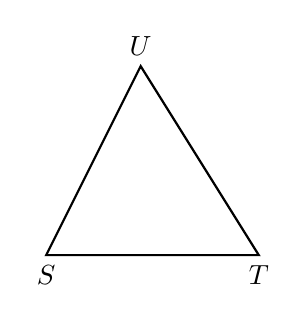
\begin{tikzpicture}[scale=0.3]
              \draw[thick] (0,0)node[below]{$S$}--
                (9,0) node[below]{$T$}--
                (4,8) node[above]{$U$}--cycle;
            \end{tikzpicture}
            \end{center}

        Lesson: Area of a circle, $\pi$, decimals, powers of ten, rounding \par \medskip
        Extension: Significant figures
    \end{frame}

\section{1.10 Precision \hfill 21 September}
\begin{frame}{Learning Target: I can quantify error in calculations}
    {CCSS: HSG.CO.A.1 Know precise geometric definitions \hfill \alert{1.10 Wednesday 21 Sept}}
        Do Now: Find the area of a circle with radius $b=10$ centimeters, rounding to the nearest whole number. \par
        circle image \\

        Lesson: Percent error formula \par \medskip
        Extension: Confidence intervals
    \end{frame}  

\section{1.11 Review \hfill 22 September}
\begin{frame}{Learning Target: I can study together with my classmates}
    {CCSS: HSG.CO.A.1 Know precise geometric definitions \hfill \alert{1.11 Thursday 22 Sept}}
        Do Now: Find the area of a circle with radius $b=10$ centimeters, rounding to the nearest whole number. \par
        circle image \\

        Lesson: Peer review, notebook check, homework inventory due \par \medskip
        \alert{Unit test tomorrow}
    \end{frame} 

\begin{frame}{Groupwork review for \alert{test tomorrow}}
    {``Roundtable'' of four students, with four topics assigned}
    \begin{block}{Geometry skills to study / teach}
        \begin{enumerate}
        \item Conventions: terminology, notation, diagramming
        \item Modeling situations with algebra
        \item Perimeter and special shapes: 
        \begin{itemize}
        \item Scalene, isosceles, and equilateral $\triangle$s
        \item Squares, rectangles, parallelograms, trapezoids, rhombuses, kites \par 
        (quadrilateral side $\cong$s will be marked)
        \end{itemize}
        \item Solving algebraic equations for one variable
    \end{enumerate}
    \end{block}
    \end{frame}
    
\section{1.12 Unit test: Segments, length, area \hfill 23 September}
\begin{frame}{Learning Target: I can quantify length and area}
    {CCSS: HSG.CO.A.1 Know precise geometric definitions \hfill \alert{1.12 Friday 23 Sept}}

        \alert{Unit test}
    \end{frame} 
    
    
\end{document}